% !TEX program = xelatex
\documentclass[11pt, aspectratio=169]{beamer}
\usetheme{metropolis}
\useoutertheme{metropolis}
\useinnertheme{metropolis}
\usecolortheme{metropolis}
\usefonttheme{professionalfonts} 

\usepackage{kotex}
\usepackage{tikz} 
\usepackage{graphicx, caption, hyperref, fontawesome5}

% [수식 및 폰트 설정 - 기존 파일 그대로 유지]
\usepackage{amsmath}
\usepackage[math-style=ISO, bold-style=ISO]{unicode-math}
\usefonttheme{professionalfonts}

% [캡션 스타일 설정]
% 1. 캡션 폰트: 굵게(bold) 제거(\mdseries), 크기는 약간 작게(\small)
\setbeamerfont{caption}{series=\mdseries, size=\small}
\setbeamerfont{caption name}{series=\mdseries}
% 2. 캡션 번호 붙이기 (Figure 1: ...)
\setbeamertemplate{caption}[numbered]
% 3. 캡션 레이블 구분자 (Figure 1. Caption)
\setbeamertemplate{caption label separator}[period]

% [중요] 그림 경로 수정 (슬라이드 폴더 기준 2단계 위로)
\graphicspath{ {./} {../../assets/} {../assets/} }

%%%%%%%%%%%%%%%%%%%%%%%%%%%%%%%%%%%%%%%%%%%%%
%%%%%%%%%%%%%%%%%%%%%%%%%%%%%%%%%%%%%%%%%%%%%%

\title{Communication Theory - 2026}
\subtitle{Chapter 2. Signals and Signal Space}
\date{\today}
\author{
    이 경 근 \\
    {\tiny
        % \texorpdfstring{문서에 보일 내용}{PDF 속성에 들어갈 텍스트(특수문자 제외)}
        \texorpdfstring{\raisebox{-0.1ex}{\scalebox{0.85}{\faEnvelope}}}{} \href{mailto:infosec@knu.ac.kr}{infosec@knu.ac.kr} \quad 
        \texorpdfstring{\scalebox{0.9}{\faLinkedin}}{} \scalebox{0.9}{\href{https://www.linkedin.com/in/Kenny-0633-Lee}{Kenny-0633-Lee}}
    }
}
\institute{EE / KNU}

%%%%%%%%%%%%%%%%%%%%%%%%%%%%%%%%%%%%%%%%%%%%%
%%%%%%%%%%%%%%%%%%%%%%%%%%%%%%%%%%%%%%%%%%%%%
% [Font Settings] Project-Local Fonts (Perfect Stability)
\usepackage{fontspec}

% 시스템 폰트가 아니라, ./fonts 폴더의 파일을 직접 사용합니다.
\setmainfont{NotoSansKR-Regular.ttf}[
    Path = ../../fonts/,             % 폰트 파일 위치
    BoldFont = NotoSansKR-Bold.ttf,
    AutoFakeSlant = 0.2          % 이탤릭 강제 구현
]

\setsansfont{NotoSansKR-Regular.ttf}[
    Path = ../../fonts/,
    BoldFont = NotoSansKR-Bold.ttf,
    AutoFakeSlant = 0.2
]

\setmainhangulfont{NotoSansKR-Regular.ttf}[
    Path = ../../fonts/,
    BoldFont = NotoSansKR-Bold.ttf,
    AutoFakeSlant = 0.2
]

\setsanshangulfont{NotoSansKR-Regular.ttf}[
    Path = ../../fonts/,
    BoldFont = NotoSansKR-Bold.ttf,
    AutoFakeSlant = 0.2
]

% 수식 폰트 설정
\setmathfont{Fira Math}
\setmathfont[range={up, bfup}, Scale=MatchLowercase, Path = ../../fonts/]{NotoSansKR-Regular.ttf}
\setmathfont[range={it, bfit}, Scale=MatchLowercase, FakeSlant=0.2, Path = ../../fonts/]{NotoSansKR-Regular.ttf}
%%%%%%%%%%%%%%%%%%%%%%%%%%%%%%%%%%%%%%%%%%%%%

\begin{document}

% 1. 표지
\begin{frame}[plain]
    \titlepage
\end{frame}

% 2. 강의 목차
% \begin{frame}
%     \frametitle{Table of Contents}
%     \tableofcontents
% \end{frame}

% Definitions : Signals and Systems
\begin{frame}{Definitions: Signals and Systems}
    \begin{block}{\fbox{Signals}}
        A signal is a set of information or data. \\
        Examples: Audio signals, video signals, sensor data, etc.\\
        In all these examples, the signals are functions of the independent variable \textbf{time $t$}.
    \end{block}
    \vspace{0.2cm}
    \begin{block}{\fbox{Systems}}
        Signals may be processed further by systems, which may modify them or extract additional infromation from them. \\
        For example, an antiaircraft radar system processes the received signals (inputs) to determine the position and velocity of an aircraft (outputs). \\
        Thus, a system is an entity that processes signals (\textbf{inputs}) to yield another set of signals (\textbf{outputs}). \\
        More examples: Amplifiers, filters, modulators, demodulators, etc.
    \end{block}
\end{frame}

% 2.1 신호의 크기
\begin{frame}
    \frametitle{Size of Signal}
    \begin{columns}
        % [왼쪽 컬럼] 그림 (a), (b) 배치 및 통합 캡션
        \begin{column}{0.45\textwidth}
            \begin{figure}
                \centering
                % (a) Energy Signal
                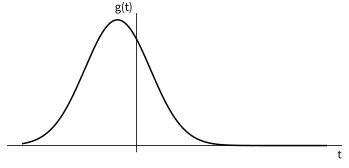
\includegraphics[width=0.8\textwidth]{fig_ch02_energy_sig.pdf} \\
                \vspace{-0.2cm} {\footnotesize (a) Signal with finite energy} \\
                \vspace{0.3cm} % (a)와 (b) 사이 간격
                
                % (b) Power Signal
                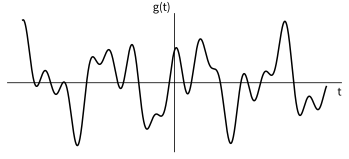
\includegraphics[width=0.8\textwidth]{fig_ch02_power_sig.pdf} \\
                \vspace{-0.2cm} {\footnotesize (b) Signal with finite power}
                
                % [통합 캡션] 맨 아래에 위치, 굵은 글씨 없음
                \caption{Examples of signals.} 
            \end{figure}
        \end{column}

        % [오른쪽 컬럼] 텍스트 설명
        \begin{column}{0.55\textwidth}
            \begin{block}{Energy Signal}
                A signal is said to be an energy signal if its energy is finite and its average power is zero.
                \[
                E = \int_{-\infty}^{\infty} |x(t)|^2 dt < \infty, \quad P = 0
                \]
            \end{block}
            %\vspace{0.1cm}
            \begin{block}{Power Signal}
                A signal is said to be a power signal if its average power is finite and its energy is infinite.
                \[
                P = \lim_{T \to \infty} \frac{1}{2T} \int_{-T}^{T} |x(t)|^2 dt < \infty, \quad E = \infty
                \]
            \end{block}
        \end{column}
    \end{columns} 
\end{frame}

%%% Sample Frames %%%
\begin{frame}{Overview}
    \begin{itemize}
        \item \textbf{Basic Signals:} 단위 계단 함수 $u(t)$와 델타 함수 $\delta(t)$
        \item \textbf{Signal Operations:} 시간 이동(Shifting)과 스케일링(Scaling)
        \item \textbf{Correlation:} 신호의 유사도(Similarity) 측정
    \end{itemize}
\end{frame}

% 3. 기본 신호 (Unit Step)
\begin{frame}{1. Basic Signals: Unit Step Function}
    \begin{columns}
        \begin{column}{0.6\textwidth}
            \centering
            % Python(ch02_signals.py)에서 생성한 그림
            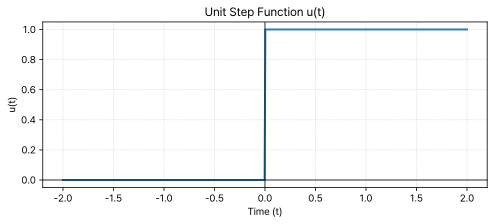
\includegraphics[width=\textwidth]{fig_ch02_unit_step.pdf}
        \end{column}
        \begin{column}{0.4\textwidth}
            \begin{block}{Definition}
                \[
                u(t) = \begin{cases} 
                1, & t \ge 0 \\ 
                0, & t < 0 
                \end{cases}
                \]
            \end{block}
            \vspace{0.2cm}
            \textbf{Key Property:} \\
            시스템의 스위칭 동작(Switching)을 수학적으로 모델링할 때 사용됨.
        \end{column}
    \end{columns}
\end{frame}

% 4. 신호의 연산 (Shifting & Scaling)
\begin{frame}{2. Signal Operations: $x(at - b)$}
    \begin{columns}
        \begin{column}{0.55\textwidth}
            \centering
            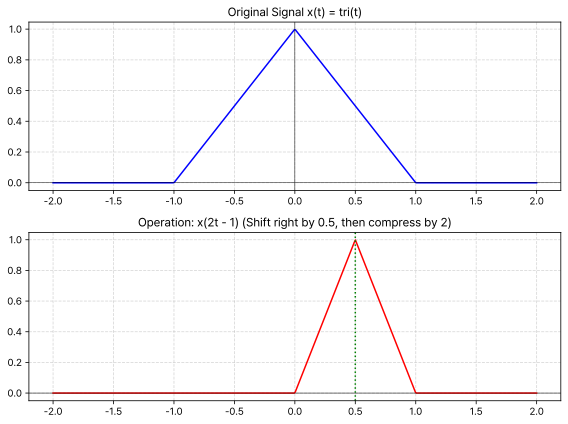
\includegraphics[width=\textwidth]{fig_ch02_operations.pdf}
        \end{column}
        \begin{column}{0.45\textwidth}
            \small
            \textbf{해석 순서 (Order of Operations):}
            \begin{enumerate}
                \item \textbf{Shifting:} $t \rightarrow t - t_0$ \\
                (Right if $t_0 > 0$)
                \item \textbf{Scaling:} $t \rightarrow at$ \\
                (Compression if $a > 1$)
            \end{enumerate}
            
            \vspace{0.3cm}
            \begin{alertblock}{Caution}
                $x(2t - 1)$은 $x(t)$를 1만큼 이동 후 2배 압축하는 것이 아님! \\
                $\rightarrow x(2(t - 0.5))$로 생각해야 함.
            \end{alertblock}
        \end{column}
    \end{columns}
\end{frame}

% 5. 상관관계 (Correlation)
\begin{frame}{3. Signal Correlation}
    \centering
    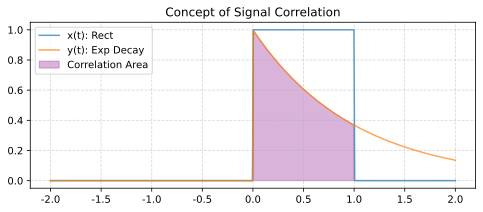
\includegraphics[width=0.7\textwidth]{fig_ch02_correlation.pdf}
    
    \vspace{0.3cm}
    \begin{block}{Correlation Coefficient ($C_n$)}
        두 신호가 얼마나 닮았는가? (Measure of Similarity)
        \[
        \rho = \frac{\int x(t) y^*(t) dt}{\sqrt{E_x E_y}}
        \]
    \end{block}
    \small \textit{그래프의 보라색 영역(Overlap)이 넓을수록 상관관계가 높습니다.}
\end{frame}

% 6. 마무리
\begin{frame}{Summary}
    \begin{itemize}
        \item \textbf{Unit Step $u(t)$:} 인과성(Causality) 표현의 핵심
        \item \textbf{Operations:} $x(at-b)$ 꼴의 변환을 자유자재로 다뤄야 함
        \item \textbf{Correlation:} 통신 시스템에서 수신 신호를 검출(Detection)하는 기본 원리
    \end{itemize}
\end{frame}

\end{document}